\documentclass{beamer}

\usepackage[utf8]{inputenc}
\usepackage{hyperref}

\usetheme{Berkeley}
\beamertemplatenavigationsymbolsempty
\setbeamertemplate{headline}{}
 
\title{FoodChain-Lab Einführung}
\date{}
 
\begin{document}
\maketitle

\section{FoodChain-Lab Konzepte 1}
\begin{frame}
	\begin{itemize}
		\item \textbf{Delivery (Lieferung)}: Wird von A nach B an einem bestimmten Datum versendet. Eine Lieferung kann Folgelieferungen und vorhergehende Lieferungen haben (z.B. Erdbeer-Lieferung -$>$ Erdbeerkuchen-Lieferung).
		\item \textbf{Station}: Lebensmittelunternehmen oder Person, das/die Lieferungen empfängt und/oder versendet.
		\item \textbf{Trace}: Pfad den eine Kontamination nehmen kann. Eine Station/Lieferung "B" ist auf dem \textbf{Forward Trace} von einer Station/Lieferung "A", falls sich eine Kontamination über das Liefernetz von "A" nach "B" ausbreiten kann. Wenn "B" auf dem \textbf{Forward Trace} von "A" ist, dann ist "A" auf dem \textbf{Backward Trace} von "B".
	\end{itemize}
\end{frame}

\section{FoodChain-Lab Konzepte 2}
\begin{frame}
	\begin{itemize}
		\item \textbf{Weight (Gewicht)}: Gewichte werden an Stationen/Lieferungen vergeben, die in einen Ausbruch involviert sind (z.B. ein Restaurant in dem Kunden infiziert wurden). Verschiedene Gewichte können benutzt werden um Unterschiede zwischen den involvierten Stationen/Lieferungen zu modellieren (z.B. höheres Gewicht = größere Wahrscheinlichkeit, dass Station/Lieferung involviert ist).
		\item \textbf{Cross Contamination (Kreuzkontamination)}: Bei Stationen werden ausgehende Lieferungen von eingehenden Lieferungen kontaminiert. Falls auf Lieferungen angewendet, kontaminieren die gewählten eingehenden Lieferungen einer Station ihre Folgelieferungen.
		\item \textbf{Score}: Wird auf Basis der vergebenen Gewichte und Kreuzkontamination berechnet. Soll helfen die Wahrscheinlichkeit abzuschätzen, dass eine Station/Lieferung die Quelle des Ausbruchs ist (höherer Score = höhere Wahrscheinlichkeit, dass Quelle des Ausbruchs).
	\end{itemize}
\end{frame}

\section{FoodChain-Lab Score Berechnung}
\begin{frame}
	\begin{center}
  		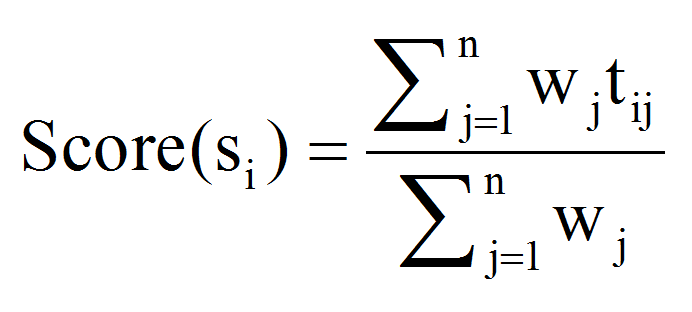
\includegraphics[height=0.3\textheight]{score.png}
	\end{center}
	\begin{itemize}
		\item $s_i$: i-te Station oder Lieferung
		\item $w_j$: Gewicht ("Weight") der j-ten Station oder Lieferung
		\item $t_{ij}$: hat einen Wert von 1, falls es einen Trace von $s_i$ nach $s_j$ gibt, ansonsten 0
		\item $n$: Anzahl aller Stationen und Lieferungen
	\end{itemize}
\end{frame}

\section{KNIME-Einführung}
\begin{frame}
	\begin{itemize}
		\item KNIME ist eine Open Source Datenanalyse-Platform, die es dem Nutzer erlaubt Daten-Pipelines (sogenannte "Workflows") zu bauen
		\item Ein Workflow wird erstellt indem Knoten aus dem \textbf{Node Repository} in den \textbf{Workflow Editor} gezogen und verbunden werden (\url{https://tech.knime.org/workbench}).
		\item Knoten sind Datenverarbeitungs-Einheiten mit Ein- und/oder Ausgabe-Ports.
		\item Daten können über eine Verbindung vom Ausgabe-Port zum Eingabe-Port eines anderen Knotens übermittelt werden.
		\item Ausführlicher KNIME quickstart guide: \url{https://tech.knime.org/files/KNIME_quickstart.pdf}.
		\item Einführungsvideo zu KNIME: \url{https://www.youtube.com/watch?v=ft7Ksgss3Tc}.
	\end{itemize}
\end{frame}

\section{Verfügbare Knoten}
\begin{frame}
	\begin{center}
  		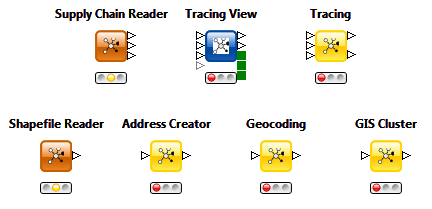
\includegraphics[height=0.4\textheight]{1.png}
	\end{center}
	\begin{itemize}
		\item Die detaillierten Beschreibungen aller Knoten finden Sie in der \textbf{Node Description} in KNIME (\url{https://tech.knime.org/workbench}).
		\item Eingehende und ausgehende Daten sind entweder Daten-Tabellen (repräsentiert durch Dreiecke an den Knoten) oder Bilder (repräsentiert durch grüne Quadrate). Diese Datentypen werden standardmäßig in KNIME verwendet (z.B. beim \textbf{Row Filter} oder \textbf{Image Port Writer}), so dass KNIME-Knoten ebenfalls in FoodChain-Lab-Workflows verwendet werden können.
	\end{itemize}
\end{frame}
 
\section{Tracing}
\begin{frame}
	\begin{center}
  		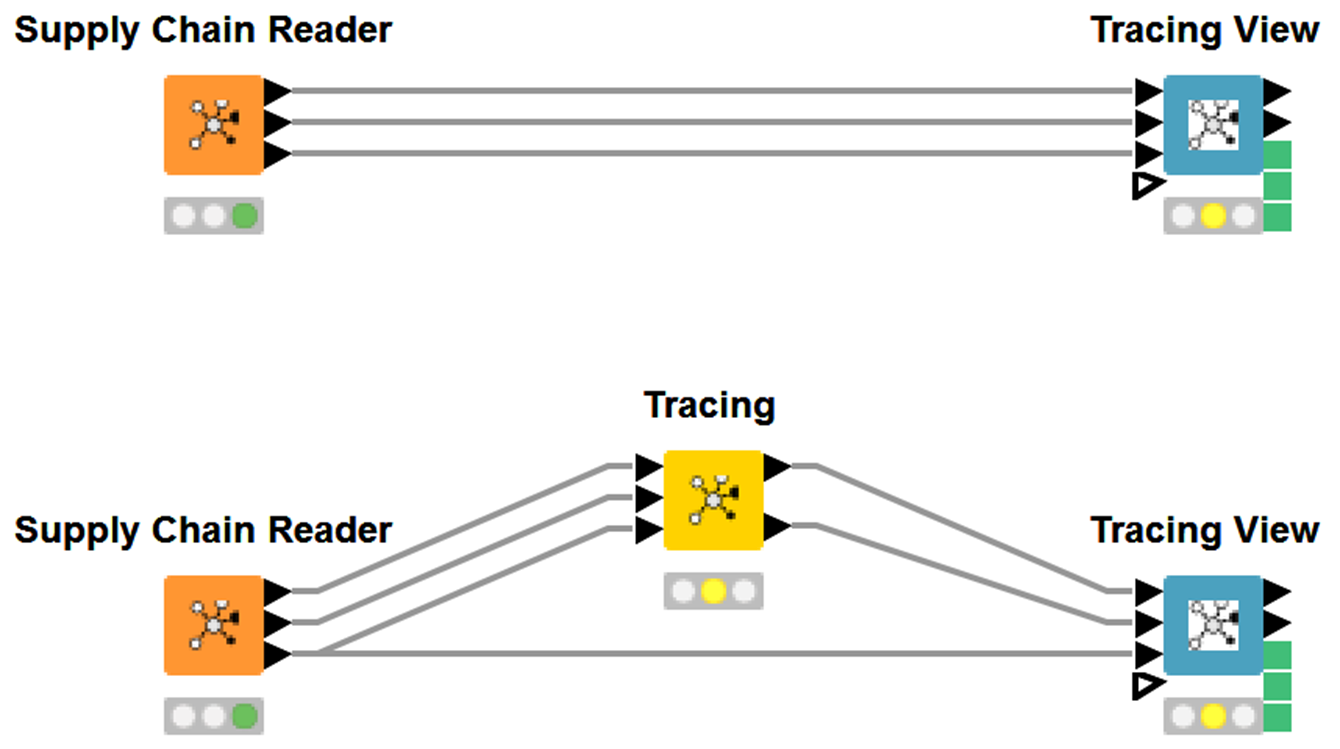
\includegraphics[height=0.4\textheight]{2.png}
	\end{center}
	\begin{itemize}
		\item Daten zu Lieferketten werden aus der internen Datenbank mit dem \textbf{Supply Chain Reader} in den Workflow geladen.
		\item Diese Daten können mit dem \textbf{Tracing View} visualisiert werden. Außerdem kann der \textbf{Tracing View} auch ein Tracing auf den Daten durchführen.
		\item Der \textbf{Tracing}-Knoten erlaubt es ein Tracing ohne Visualisierung durchzuführen (z.B. als Vorverarbeitungsschritt für den \textbf{Tracing View}).
	\end{itemize}
\end{frame}

\section{Verwenden von Geodaten}
\begin{frame}
	\begin{center}
  		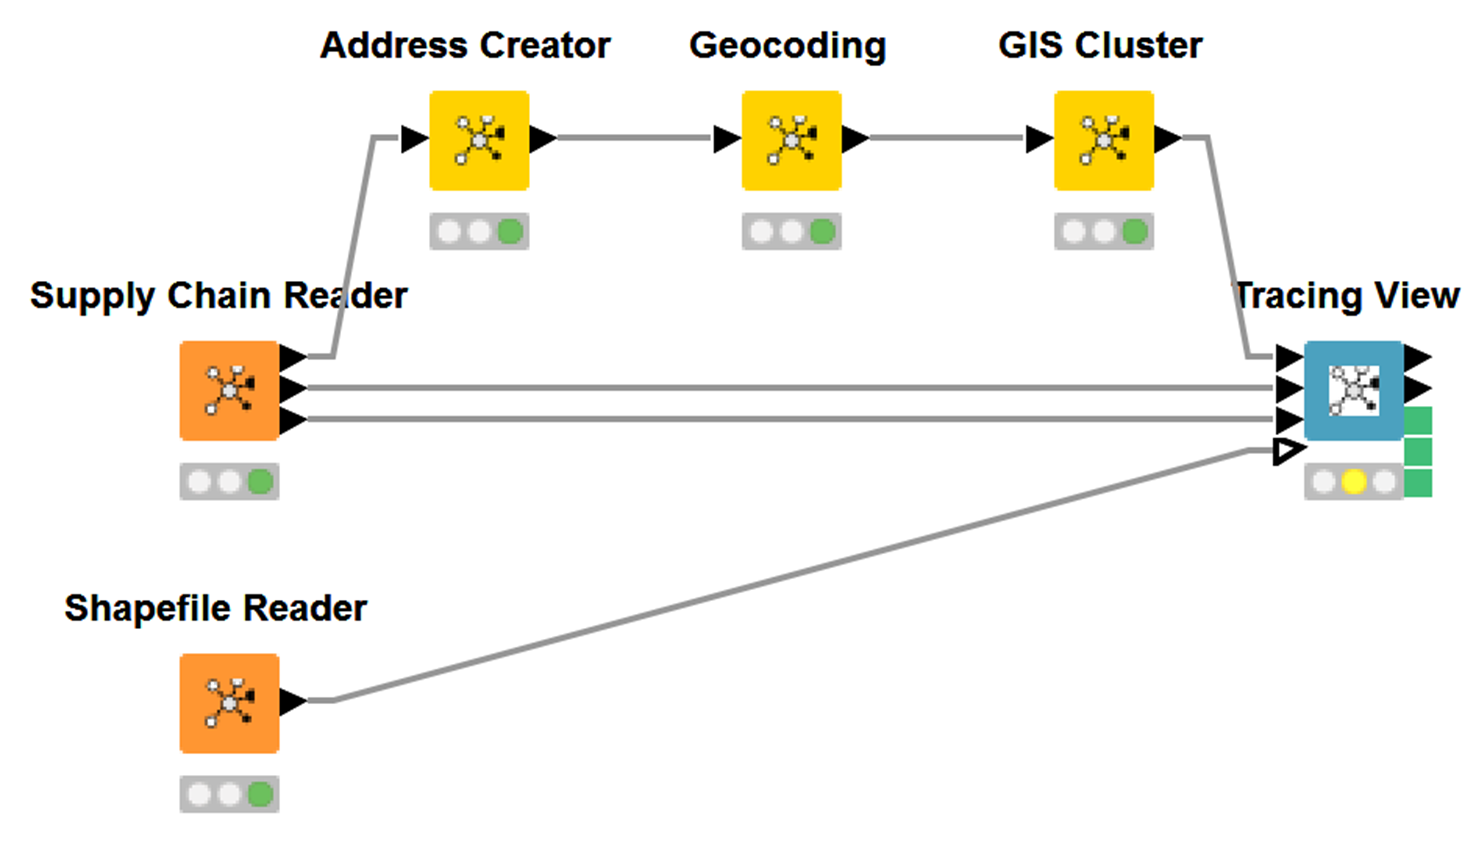
\includegraphics[height=0.5\textheight]{3.png}
	\end{center}
	\begin{itemize}
		\item Der \textbf{Geocoding} Knoten ermittelt anhand von Adressen die geographische Breite und Länge.
		\item Mit diesen Daten können dann im \textbf{GIS Cluster}-Knoten sogenannte Cluster (regionale Zusammenhänge) errechnet werden.
		\item Der Tracing View kann die Lieferketten auf einer Landkarte visualisieren, welche mit dem \textbf{Shapefile Reader} eingelesen wird.
	\end{itemize}		
\end{frame}

\end{document}